%% ================================================================================
%% This LaTeX file was created by AbiWord.                                         
%% AbiWord is a free, Open Source word processor.                                  
%% More information about AbiWord is available at http://www.abisource.com/        
%% ================================================================================

\documentclass[a4paper,portrait,12pt]{article}
\usepackage[latin1]{inputenc}
\usepackage{calc}
\usepackage{setspace}
\usepackage{fixltx2e}
\usepackage{graphicx}
\usepackage{multicol}
\usepackage{minted}
\usepackage{listings}
% \usepackage{csquotes}
%\usepackage[normalem]{ulem}
%% Please revise the following command, if your babel
%% package does not support en-US
%\usepackage{babel}
\usepackage{color}
\usepackage{hyperref}
 
\begin{document}

\setlength{\oddsidemargin}{0.9847in-1in}
\setlength{\textwidth}{\paperwidth - 0.9847in-0.9847in}

\author{Ovidiu Popoviciu, 2036725}
\date{17th November 2017}
\title{Twitter Event Detection - MSci}
\maketitle

%%%%%%%%%%%%%%%%%%%%%%%%%%%%%%%%%%%%%%%%%%%%%%%%%%%%%%%%%%%%%%%%%%%%%%%%%%%%%%%%%%
\section{Introduction}

Event detection in social media is a challenging task.
This is due to the amount of tweets (approx. 500 million tweets per day in 2016 \cite{tweetStats}), amount of relevant tweets is very small (90\% are junk), limitations with the API (until recently \cite{twitterPremium}), importance of events and scalability issues, spelling and grammar mistakes in tweet body as well abbreviations and acronyms are difficult to identify.\\
The objective of this work is to evaluate a stage of the event detection process initially defined by McMinn et al. \cite{McMinn2013} \cite{McMinn2015} on a collection of tweets.

%%%%%%%%%%%%%%%%%%%%%%%%%%%%%%%%%%%%%%%%%%%%%%%%%%%%%%%%%%%%%%%%%%%%%%%%%%%%%%%%%%
\section{Approach}
\cite{McMinn2013} \cite{McMinn2015}

Two approaches are defined, each executed after the clustering stage provided by McMinn et al. \cite{McMinn2013}.

Following the work of McMinn et al. \cite{McMinn2013}, the steps taken in the processing of the dataset are:
\begin{itemize}
	\item Gathering data. This was already done for us, and the dataset was shared from the previous study.
	\item Preprocessing. The dataset was already pre-processed. Tweets were parsed, tagged and filtered. All that remained were the relevant tweets with tokens that might relate back to an event.
	\item Clustering. The data set contained clusters of tweets already defined, through the use of an Inverted Index and tweets grouped together using weight cosine similarity score.
	\item Burst Detection. Check for temporal bursts of a named entity in a window period of minutes to hours. This step was completed in conjunction with event merging.
	\item Cluster Identification. In McMinn et al. \cite{McMinn2013} evaluation program, clusters are already considered to map to a specific event since clusters with no named entities have been removed.
	\item Event Merging. Merging events with multiple entities since  Discussion of this work is focused on this step.
\end{itemize}

The dataset provided has been pre-processed and organised into clusters.
The missing stages, which is provided in this work, is cluster identification and event merging.
The two approaches discussed here are:
\begin{enumerate}
	\item Filtering.
	      Identify clusters which have limited or no relevance to any important events and remove them.
	      This step may be considered as an enhancement of Cluster Identification.
	      The goal was to see whether removing clusters with a specific number of tweets might reduce the resulting data set returned and thus increase precision of the system.
	\item Merging.
	      The goal was to study whether clusters with the same named entity, lying within the same temporal burst can be considered a single event.
	      In McMinn's study, clustering of tweets was optimised performance wise by reducing the number of tweets retrieved from the Inverted Index and thus reducing the number of comparisons for each tweet to be added to a cluster.
	      Thus, we wanted to know whether multiple clusters with the same event (and same named entity) have been created within a specific time period and if merging of these clusters would have a positive effect on the performance of the system.
\end{enumerate}

The evaluation and discussion of the two approaches are dicusses in Section \ref{section-eval} and Section \ref{section-discussion}.

%%%%%%%%%%%%%%%%%%%%%%%%%%%%%%%%%%%%%%%%%%%%%%%%%%%%%%%%%%%%%%%%%%%%%%%%%%%%%%%%%%
\section{Code Description}
The code has been written in Java, due its object-oriented structure, efficiency and ability to handle 64-bit Integer values available from the data set.
UML diagrams and descriptions are provided.\\

\begin{figure}[h!]
	\centering
	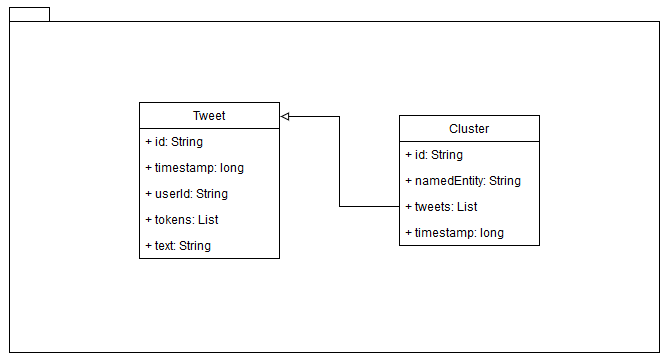
\includegraphics[width=0.5\linewidth]{images/modelUML.png}
	\caption{UML model classes}
	\label{fig:modelUML}
\end{figure}

Initially, two model classes have been defined, as seen in Figure \ref{fig:modelUML}. The first class, Tweet, contains the appropriate fields for identifying a tweet, such as: tweet ID, timestamp, user ID, parsed tweet tokens and the body text of the tweet.
Additionally, a second model class defined is Cluster, which references the previous class tweet. Cluster class contains a list of tweets with the same properties and is defined by a cluster ID, by the named entity which are identified by all the tweets and a timestamp which, we'll see in the next paragraphs, will hold the centroid time of all tweets in that specific cluster.\\

The data set is read from local disk through an instance of IOProcessor, which is an interface for reading data.
Since the data set is in CSV format, a class CSVProcessor implementing the IOProcessor interface has been defined.
It provides methods for reading CSV cluster files and instantiating model classes to be used in the logic of the system.
Diagram for Processor classes can be seen in Figure \ref{fig:processorUML}. \\

\begin{figure}[h!]
	\centering
	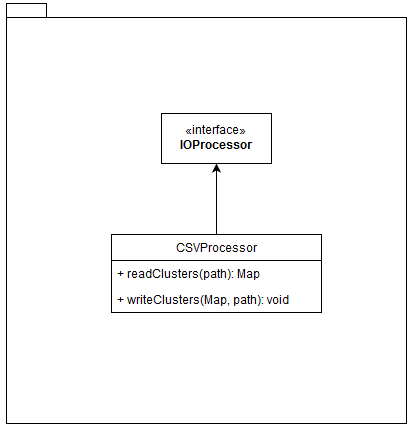
\includegraphics[width=0.5\linewidth]{images/processorUML.png}
	\caption{UML IO processor classes}
	\label{fig:processorUML}
\end{figure}

Data is read and processed as streams of Cluster objects on which multiple sequential operations can be applied.
ClusterFilter is an interface that can be extended to add more available operations. The available operations, as seen in \ref{fig:filterUML}, are:
\begin{itemize}
	\item NumberOfTweetsFilter - is a class that filters the cluster by a set number of tweets.
	\item CentroidCalculationFilter - provides a method for calculating the centroid time for each cluster within the stream.
	\item MergeNamedEntityFilter - is a filter that merges clusters with the same named entities. A time difference can be set that merges cluster with their centroid time within the same time difference.
\end{itemize}

\begin{figure}[h!]
	\centering
	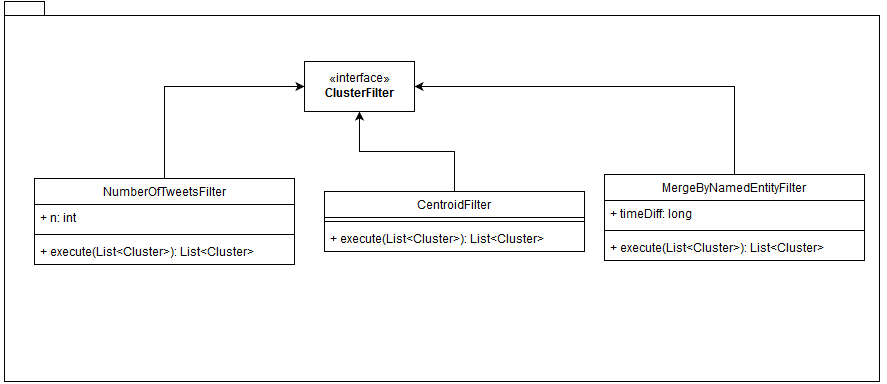
\includegraphics[width=0.7\linewidth]{images/filterUML.png}
	\caption{UML filter classes}
	\label{fig:filterUML}
\end{figure}

Each one of these filters can be applied in any sequence and the entire code can be run into a class containing the main function.
Once all the operations are applied on the stream, the clusters are written back to the file, with the help of CSVProcessor.

\begin{figure}[h!]
	\centering
	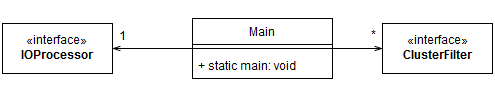
\includegraphics[width=0.7\linewidth]{images/mainUML.png}
	\caption{UML Main class}
	\label{fig:mainUML}
\end{figure}

The evaluation stage was the same as McMinn et al. \cite{McMinn2013}, and used a python script to evaluate the CSV files containing the clusters against crowd gathered events.
Additionally, due to the repetitive nature of the approaches, evaluating each CSV cluster file, gathering of results and manually pasting them into a data processor (e.g. Excel) may take a long time.
For this problem, a Gradle tasks was implemented that automatically run the two Java programs and generate all the files using only one command.
To gather the results from the output of the Python evaluation program, a NodeJS script has been developed that runs the evaluation automatically and creates a JSON containing the respective results for the analysis.
For example, all the results for the 1 day dataset with the filtering approach applied, would be contained within a single JSON file 1day-filtered.json.
The JSON schema is as follows:
\begin{lstlisting}[caption=JSON Schema Example, label=json-schema]
[{
    "file": "0",
    "data": {
        "events": {
            "total": 506,
            "detected": 19
        },
        "clusters": {
            "total": 8829,
            "matched": 120
        },
        "stats": {
            "recall": 0.038,
            "precision": 0.014,
            "fmeasure": 0.02
        }
    }
},
...
]
\end{lstlisting}

Once all files have been evaluated, the JSON schema is loaded into a JavaScript file, included into an HTML file which will display the results in a nice format using frappe-charts package (TODO: Add link to frappe-charts).
The source code is available in the source zip as well as with the instructions on how to run the code.


%%%%%%%%%%%%%%%%%%%%%%%%%%%%%%%%%%%%%%%%%%%%%%%%%%%%%%%%%%%%%%%%%%%%%%%%%%%%%%%%%%
\section{Evaluation}
\label{section-eval}

The evaluation of the two approaches relies on two measures:
\begin{itemize}
	\item \textbf{Precision}. This measure signifies the proportion of the clusters that are relevant, which relate to an event.
	      This measure is the opposite of the fraction of data which is considered \"junk\".
	\item \textbf{Recall}. Defines the fraction of clusters that were found to be relevant.
	      This measure cannot increase further than its value from the initial clusters provided since the data set is fixed.
	\item \textbf{F-Measure}.
\end{itemize}

Since recall precision cannot increase, then the evaluation focuses on increased precision with minimal negative impact to recall.

\begin{enumerate}
	\item Data collection discussion
	\item Explain evaluation measures and report the measures
	\item critically comment on results
\end{enumerate}

\begin{figure}[h!]
	\centering
	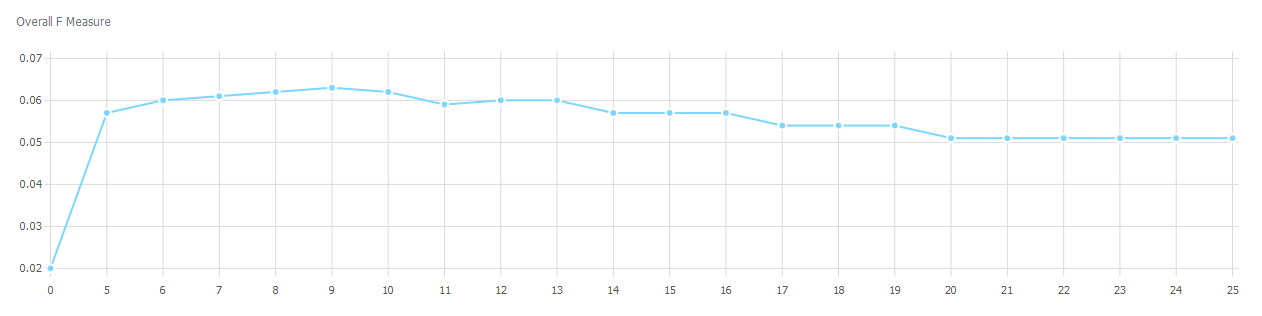
\includegraphics[width=\linewidth]{images/1day-filtered-f-measure.png}
	\caption{1 Day Filtered - F-Measure}
	\label{fig:1day-filtered-f-measure}
\end{figure}

%%%%%%%%%%%%%%%%%%%%%%%%%%%%%%%%%%%%%%%%%%%%%%%%%%%%%%%%%%%%%%%%%%%%%%%%%%%%%%%%%%
\section{Discussion}
\label{section-discussion}
\begin{enumerate}
	\item scalability, usability, effectiveness, efficiency, etc.
	\item applications of the method
	\item justify with data/information
\end{enumerate}

%%%%%%%%%%%%%%%%%%%%%%%%%%%%%%%%%%%%%%%%%%%%%%%%%%%%%%%%%%%%%%%%%%%%%%%%%%%%%%%%%%
\section{Traffic Event Detection}
\subsection{Problem Statement}
\subsection{Proposed Solution}
\subsection{Discussion}

%==============================================annotated bibliography
\newpage
\nocite{*}
\bibliographystyle{plain}
\bibliography{bibliography}

\end{document}
